\chapter{Related work}\label{Chap:relatedwork}

% The relevant background knowledge has been reviewed to design a model for predicting earthquake occurrences.
There is an overview of the Earthquake disaster in~\ref{sec:Earth}. Moreover, in subsection~\ref{subsec:seismic},  Subsection~\ref{sec:EEWS} describes the earthquake early warning system (EEWS) used to monitor ground-shaking activity. Recently, it has become commonplace to employ deep learning techniques for EEWS. The popular techniques are described in detail in section~\ref{sec:DL-EEWS}. Also, the subsection ~\ref{subsec:elm} explains the method used in this research. Finally, subsection~\ref{subsec:featureExtract} emphasizes feature-extracting techniques, a vital component of deep learning techniques.  

\section{Earthquake}\label{sec:Earth}
An earthquake is an unpredictable natural disaster, but the observable phenomena during its occurrence can serve as a warning and help mitigate the resulting losses. 

Furthermore, it's important to note that the impact and behavior of earthquake disasters can significantly vary based on local geological, geotechnical, and environmental factors. 

As a result, many countries opt to develop their own earthquake monitoring and warning systems, rather than relying on models or systems established by other nations.
\subsection{Seismic waves} \label{subsec:seismic}

% Seismic waves are acoustic oscillations~\cite{salam2021earthquake} that transport energy away from their source. They are caused by natural and artificial seismic sources, such as earthquakes, volcanic eruptions, and nuclear weapons detonation, propagating throughout the Earth. A rapid release of seismic waves has occurred at the earthquake's hypocenter or its epicenter. The hypocenter is located beneath the Earth's surface, whereas the epicenter is the affected surface area directly above the hypocenter. The vertical distance between the hypocenter and the epicenter is called the focal depth.

% Additionally, seismic waves generated by an earthquake exhibit distinctive characteristics. Seismic waves are categorized into two main types: body waves and surface waves. The first waves observed by seismic sensors during an earthquake are body waves, which propagate through the interior of the Earth. The body waves are sequentially discharged as P-waves (Primary waves) and S-waves (Secondary waves). The second wave observed by seismic sensors is the surface wave. Further, surface waves can cause damage during earthquakes. So, it is worth noting that surface waves can still inflict significant damage during earthquakes \cite{chiang2022neural}.

Seismic waves are acoustic oscillations that transport energy away from their source~\cite{salam2021earthquake}. They are caused by natural and artificial seismic sources, such as earthquakes, volcanic eruptions, and nuclear weapons detonation, propagating throughout the Earth. A rapid release of seismic waves has occurred at the earthquake's hypocenter or its epicenter. The hypocenter is located beneath the Earth's surface, whereas the epicenter is the affected surface area directly above the hypocenter. The vertical distance between the hypocenter and the epicenter is called the focal depth. The seismic waves are categorized into two main types: body waves and surface waves. 

There are two primary types of seismic waves: body waves and surface waves. The first waves observed during an earthquake are body waves, which propagate through the interior of the Earth. The body waves are sequentially discharged as P-waves (Primary waves) and S-waves (Secondary waves). The components of seismic waves are shown in Figure~\ref{fig:p-wave}. Since P-waves are the quickest seismic waves detected, they are utilized for earthquake prediction.  As their name suggests, surface waves travel along the ground's surface and are slower than body waves\cite{mousavi2020machine}.  

 
 
% Nevertheless, surface waves cause damage during earthquakes. The highest amplitude of the surface waves is named peak ground acceleration (PGA), which has a measuring unit as Gal ($1Gal = 1cm/sec^2$)~\cite{chiang2022neural}. In the case of PGA higher than 80 Gal, the human can perceive the ground shaking. Thus the warning of the earthquake will be announced. People are given a window of opportunity for evacuation due to the time lag between P-waves and surface waves. 

\subsection{Peak Ground Acceleration}
The highest amplitude of the seismic waves is named peak ground acceleration (PGA), which has a measuring unit as Gal ($1Gal = 1cm/sec^2$)~\cite{chiang2022neural}. The PGA represents the most intense ground motion experienced during an earthquake at a specific location, reflecting the severity of seismic waves propagating through the area. The human can perceive the ground shaking if the peak ground acceleration is higher than 80 Gal. Thus, The PGA can represent the level of danger of ground shaking locally \cite{chiang2022neural}.

Since P-waves are the quickest seismic waves detected, they are utilized for earthquake prediction. As their name suggests, surface waves travel along the ground's surface and are slower than body waves\cite{mousavi2020machine}. The warning of the earthquake will be announced. People are given a window of opportunity for evacuation due to the time lag between P-waves and surface waves. 

\section{The earthquake early warning system} \label{sec:EEWS}

Earthquake early warning systems (EEWS) are designed to detect the seismic pulse when an earthquake occurs and evaluate the strength of the resulting damage\cite{chiang2022neural, jozinovic2020rapid, li2018machine}. In a major incident, the EEWS will be responsible for disseminating the warning to individuals and organizations in the affected area. Therefore, citizens can evacuate to a secure location. In addition, organizations can suspend the affected services to mitigate the damage\cite{gasparini2007earthquake}. 

Installed in the earthquake-prone region, seismic sensors, the sensors used to detect ground motion, are crucial components of the EEWS. The seismometers continuously monitor the ground-shaking activity and automatically transmit data to the processing center in real time to evaluate the earthquake's intensity and characteristics. Once the earthquake has been detected and analyzed, the warning message is disseminated to the affected area's stakeholders via multiple communication channels, such as the internet, SMS, siren, and other public broadcast systems \cite{gasparini2007earthquake, allen2019earthquake}. 

The EEWS does not take the role of the prediction system that can warn an earthquake before it happens. They only detect and predict the level and characteristics of an earthquake based on the P-waves, which have a relationship with the surface wave that comes after \cite{chiang2022neural, jozinovic2020rapid, li2018machine}. This interval is made possible by the time delay between the arrival of P-waves and surface waves. So, earthquake warnings can be issued, providing people with a critical window of opportunity for evacuation \cite{gasparini2007earthquake}.

\subsection{Seismic network}
A seismic network is a system of seismic sensors distributed across a territory for recording and monitoring seismic events such as earthquakes. Such networks are required for studying Earth's seismic behavior, detecting and localizing earthquakes, and evaluating potential seismic hazards\cite{gasparini2007earthquake}. 

A seismic sensors network typically comprises the following components: 1) Seismometers are in-ground seismic sensors used to measure ground shaking\cite{wu2021crowdquake+}. 2) The Data Logger collects and records the signals the seismometers monitor in digital format\cite{chiang2022neural, jozinovic2020rapid}. 3) The communication system for transmitting collected data to the central server via the internet, satellite links, or other channels\cite{gasparini2007earthquake}. 

Therefore, these networks are essential for the study of Earth's seismic behavior, the detection and precise localization of earthquakes, and the assessment of potential seismic risks.

\subsection{Seismic wave data}
Seismic wave data are provided from seismic networks (seismic sensors networks). Moreover, this seismic data plays a crucial role in EEW systems. In brief, these data form the backbone of EEW systems, enhancing their accuracy and effectiveness in ensuring public safety during seismic events.

In addition, the seismic wave data are complex which comes from the behavior of a seismic wave that is hard to understand. This reason leads to some challenges in building the models for the EEW systems.

The seismic wave data that are recorded by seismic sensors are ground motion or ground acceleration. The recorded ground motion is time series data that consists of three channels. Figure \ref{fig:seismic-wave} depicts the three motion channels as $NS$, $EW$, and $Z$, which correspond to north-south, east-west, and up-down directions of ground movement, respectively. The $NS$ and $EW$ channels detect the horizontal displacement of the ground along the north-south and the east-west axis, accordingly. While The $Z$ channel records the ground's vertical motion~\cite{chiang2022neural}. 
\begin{figure}[ht]
    \centering
    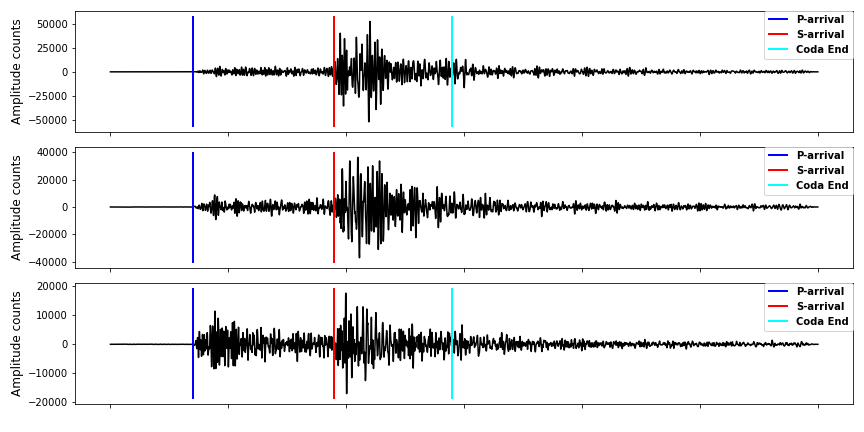
\includegraphics[width=0.9\textwidth]{img/3ch.png}
    \caption{Seismic wave that consists of P-wave and S-wave}
    \label{fig:seismic-wave}
\end{figure}

While Figure \ref{fig:seismic-wave} displays a single ground-shaking event recorded by a seismic sensor, it's important to note that during an earthquake event, seismic waves generate varying degrees of ground motion at the local level. These variations are influenced by geological factors unique to the area, such as local subsurface conditions, soil types, and the presence of geological fault lines. Consequently, different areas exhibit distinct seismic wave characteristics.
 
% Moreover, in classifying whether earthquakes happen, the three channels of P-waves are critical data. So, extracting critical features and classifying P-waves poses a challenge for models within Earthquake Early Warning (EEW) systems, as observed in previous studies\cite{chiang2022neural}. 

In classifying whether earthquakes happen, the three channels of P-waves are critical data. These waves can cross through the medium more rapidly than the rest~\cite{chiang2022neural, allen2019earthquake}. The EEWS uses these data for assessment before disseminating the earthquake incident to the affected area to prepare for coping and reducing the losses~\cite{chiang2022neural}. 

% The EEWS uses these data for assessment before disseminating the earthquake incident to the affected area to prepare for coping and reducing the losses \cite{chiang2022neural}. 

% Classification of ground shaking is essential to work in earthquake monitoring. The earthquake early warning (EEW) systems are the systems that prevent and reduce the damages caused by ground shaking generated by seismic waves \cite{chiang2022neural}. 

% The EEW systems detect initial seismic waves generated during an earthquake, called P-waves. These waves cross through the medium more rapidly than destructive S-waves and surface waves \cite{chiang2022neural, allen2019earthquake}. Therefore, the warning system can alert early to areas that may encounter strong ground shaking.

Various studies about the EEWS propose frameworks using P-waves to classify the severity scale of ground motions or peak ground acceleration~\cite{chiang2022neural, hsu2013rapid, yanwei2021deep, gasparini2007earthquake}. 

Nevertheless, deep learning models have demonstrated their capability to address the complexities of such data. Consequently, numerous studies in the field of earthquake early warning (EEW) have explored approaches that leverage P-waves for classifying the severity scale of ground motions or predicting peak ground acceleration.
%%%%%%%%%%%%%%%%%%%%%%%%%%%%%%%%%%%%%%%%%%%%%%

% \section{Earthquake Early Warning System}
% Earthquake early warning systems (EEWS) are designed to detect the seismic pulse when an earthquake occurs and evaluate the strength of the resulting damage\cite{chiang2022neural, jozinovic2020rapid, li2018machine}. In a major incident, the EEWS will be responsible for disseminating the warning to individuals and organizations in the affected area. Therefore, citizens can evacuate to a secure location. In addition, organizations can suspend the affected services to mitigate the damage\cite{gasparini2007earthquake}. 

% Installed in the earthquake-prone region, seismometers, the sensors used to detect ground motion, are crucial components of the EEWS. The seismometers continuously monitor the ground-shaking activity and automatically transmit data to the processing center in real-time to evaluate the earthquake's intensity and characteristics. Once the earthquake has been detected and analyzed, the warning message is disseminated to the affected area's stakeholders via multiple communication channels, such as the internet, SMS, siren, and other public broadcast system \cite{gasparini2007earthquake, allen2019earthquake}. The EEWS does not take the role of the prediction system that can warn an earthquake before it happens. They only detect and predict the level and characteristics of an earthquake based on the P-waves, which have a relationship with the surface wave that comes after \cite{chiang2022neural, jozinovic2020rapid, li2018machine}. 

% In EEW systems, a seismic station detects and monitors seismic waves. Figure \ref{fig:EEW} shows that the EEW model approximates the damage from the ground motion by peak ground acceleration (PGA). Also, The peak ground acceleration (PGA) has a Gal unit (Unit to express the acceleration of earthquake) which $1Gal = 1cm/s^2$, and the PGA is the highest amplitude of the ground acceleration which is recorded by seismic stations \cite{chiang2022neural}.\\
%%%%%%%%%%%%%%%%%%%%%%%%%%%%%%%%%%%%%%%%%%%

\section{Deep Learning Techniques for EEWS}\label{sec:DL-EEWS}
Many studies propose methods to classify ground shaking from seismic wave data. With the increased computing power of computers and big data \cite{mousavi2019stanford}. The deep learning model has more accuracy than traditional models, therefore the Deep learning model can overcome the conventional strong-motion classification model \cite{mousavi2020machine}.

The EEW model is the model used to classify strong motion. In EEW systems, deep learning models are practical and widely used. They are excellent at recognizing patterns of P-wave signals that are followed by a decisive motion. Moreover, they can process signal data in real-time, which provides a rapid alert \cite{li2018machine}. In addition, The automatic adaptation by data of deep learning is helpful to update and improve the EEW systems continuously. Therefore, deep learning models are powerful to use in this field.

A deep learning model comprises two primary types of layers. The initial layer is the feature extractor, designed as a matrix to identify correlations and patterns within the input data. Subsequently, the decision layer takes on the role of making predictions. 

\begin{figure}[ht]
    \centering
    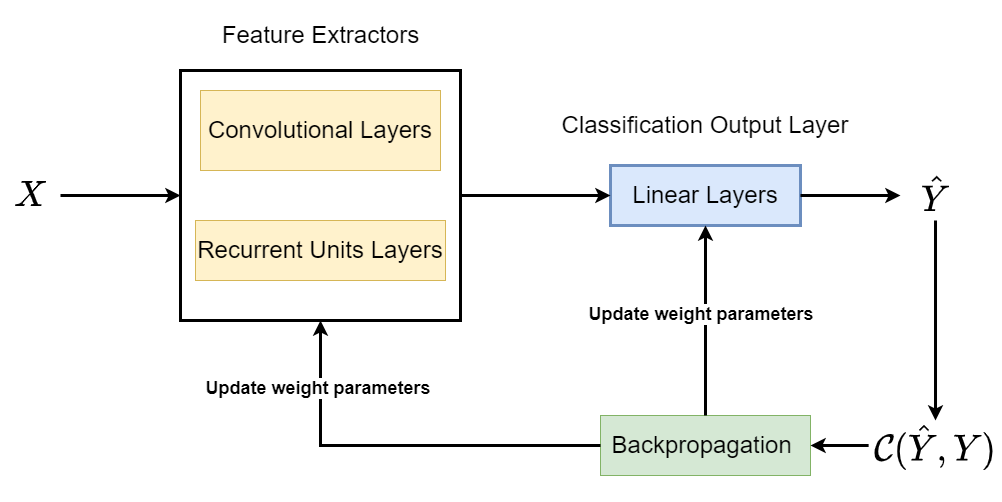
\includegraphics[width=0.9\textwidth]{img/ann.png}
    \caption{Seismic wave that consists of P-wave and S-wave}
    \label{fig:ann}
\end{figure}


Figure \ref{fig:ann} illustrates the construction of the deep learning model. It's worth noting that in Earthquake Early Warning (EEW) systems, the feature extractors commonly employed are Convolutional Neural Networks (CNN) or Recurrent Neural Networks (RNN). 

In Figure \ref{fig:ann}, $X,\ Y$ are represented as the input data and labels data respectively. $\hat Y$ refers to the prediction from the classification output layers. Also, $C$ is the cost function or error from comparing the $Y$ and $\hat Y$. The training of deep learning models can be accomplished through various methods, with backpropagation being a widely popular technique for this purpose.

\subsection{Extreme Learning Machine}\label{subsec:elm}
The Extreme Learning Machine (ELM) is a single-layer feed-forward network (SLFN). Additionally, The ELM has a structure like the deep learning model, however, its feature extractor is a random matrix called a random linear layer and a non-linear function called an activate function. The feature extractor in ELM is capable of establishing a randomized connection between the input data features, denoted as $X$, resulting in the creation of hidden features referred to as $H$. Also, the updating process in ELM is pseudo-inverse. ELM only once updates the classification output layer, while deliberately avoiding updating the feature extractor. 

% \begin{figure}[ht]
%     \centering
%     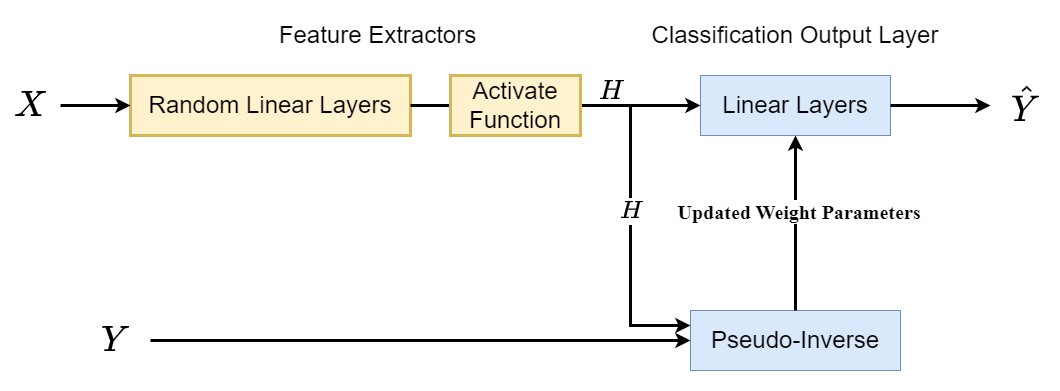
\includegraphics[width=0.95\textwidth]{img/ELM.png}
%     \caption{Extreme Learning Machine}
%     \label{fig:elm}
% \end{figure}
\begin{figure}[ht]
    \centering
    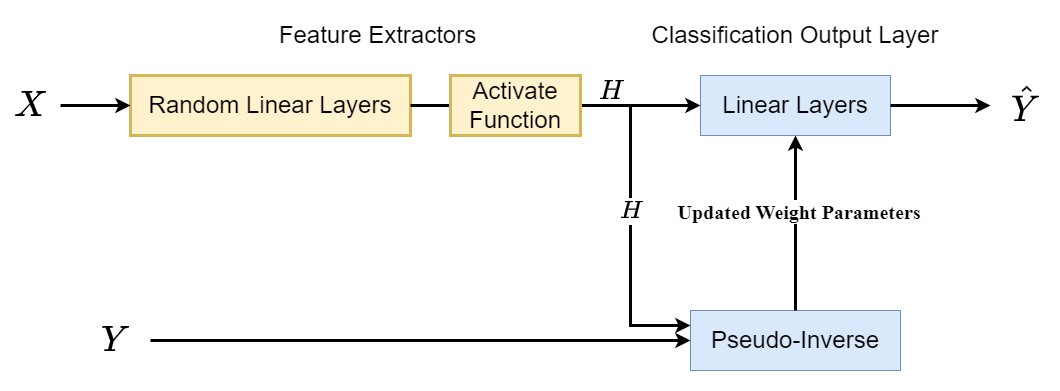
\includegraphics[width=0.95\textwidth]{img/ELM.png}
    \caption{The ELM's structure.}
    \label{fig:ELM-model}
\end{figure}

Conventional Artificial Neural Networks using forward-backward algorithms need much training time \cite{lian2013displacement}.  While, the ELM's input weight (random linear layer) is fixed, not necessary to train, and the pseudo-inverse matrix optimizes the output weight (classification output layer) of the model. So, the ELM can run faster than classical ANN while can maintain high accuracy \cite{asim2017earthquake, salam2021earthquake}. Moreover, the ELM needs the update process just one time. This reason makes the ELM consume the resources to train less than the conventional ANN.

While ELM is recognized for its superior speed compared to traditional Artificial Neural Networks (ANN), it is not appropriate for handling multi-channel time series data like seismic wave data. Hence, there are many researchers have invented new feature extractors for the ELM model.

\subsection{Feature Extracting Methods}
\label{subsec:featureExtract}
Feature extractors are components or layers in deep learning that enable the extraction of meaningful patterns from raw data. These extractors transform input data into a more compact and representative format. By learning abstract features from the data, these components can discern patterns that might not be evident to humans. The effectiveness of feature extractors plays a pivotal role in the success of deep learning models, empowering them to accomplish a diverse range of complex tasks.

\subsubsection{Convolutional  Neural Network}
Many studies \cite{chiang2022neural, jozinovic2020rapid, li2018machine, mousavi2020machine, perol2018convolutional} propose a CNN-based architecture for an EEW system. CNN is the famous structure of the deep learning model. They can auto-extract valuable features from raw seismic signals using the 1D or 2D convolution kernel and predict ground shaking from the features \cite{chiang2022neural, jozinovic2020rapid, li2018machine, mousavi2020machine, mousavi2020machine}. The CNN models can be used in real-time and accurately predict the parameters of an earthquake. Furthermore, they are faster than conventional methods, such as GMPEs, and peak displacement (Pd) \cite{chiang2022neural, jozinovic2020rapid}. Therefore, there is much research that investigates using the CNN model in an EEW system.

The research \cite{chiang2022neural} proposes a convolutional neural network to predict PGA with P-wave. It compares the result with the conventional model that uses peak displacement (Pd), which models and sets parameters with experts. Also, The research's results show that convolutional neural networks can beat the conventional model. However, deep learning models need much time and computation to learn from raw earthquake data.

\subsubsection{Echo State Network}
% \subsubsection{Feature Extracting Methods} 
\begin{figure}[ht]
    \centering
    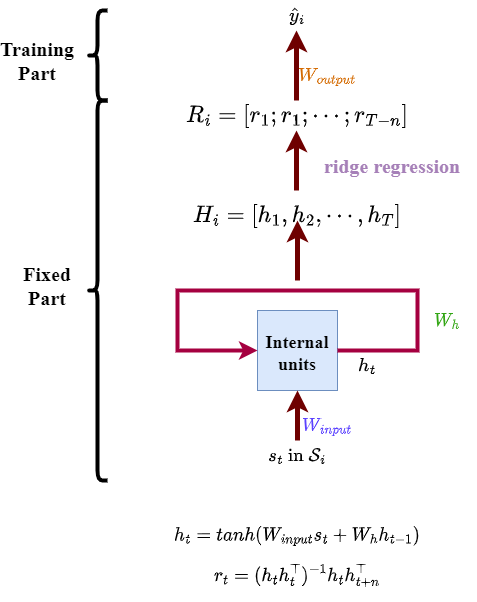
\includegraphics[width=0.6\textwidth]{img/Echo_new.png}
    \caption{The Echo State Network model consists of a fixed part and a training part.}
    \label{fig:Echo-model}
\end{figure}

The Echo State Network (ESN) is one of machine learning that has to learn with time series data like an RNN, but ESN has a recurrent part that is fixed weight \cite{cucchi2022hands}. From the fixed recurrent weight unit weight, the ESN can avoid the backpropagation process, which leads to vanishing gradient problems and consumes much time to train. Therefore, the ESN has efficient learning and fast training for time series data\cite{bianchi2020reservoir}.

The ESN model contains two parts. Figure \ref{fig:Echo-model} shows how ESN trains and predicts data. The first part is the recurrent unit layer, which applies fixed weight parameters and does not need a training process. The recurrent unit layer does not need to train the model but can represent the feature data for the supervised learning model \cite{cucchi2022hands, bianchi2020reservoir}.
%%%%%%%%%%%%%%%%%%%%%%%%%%%%%%%%%%%%%%%%%%

